\documentclass[aspectratio=169]{../latex_main/tntbeamer}  % you can pass all options of the beamer class, e.g., 'handout' or 'aspectratio=43'
\usepackage{dsfont}
\usepackage{bm}
\usepackage[english]{babel}
\usepackage[T1]{fontenc}
%\usepackage[utf8]{inputenc}
\usepackage{graphicx}
\graphicspath{ {./figures/} }
\usepackage{algorithm}
\usepackage[ruled,vlined,algo2e,linesnumbered]{algorithm2e}
\usepackage{hyperref}
\usepackage{booktabs}
\usepackage{mathtools}

\usepackage{amsmath,amssymb}

\DeclareMathOperator*{\argmax}{arg\,max}
\DeclareMathOperator*{\argmin}{arg\,min}

\usepackage{amsbsy}
\newcommand{\vect}[1]{\bm{#1}}
%\newcommand{\vect}[1]{\boldsymbol{#1}}

\usepackage{pgfplots}
\pgfplotsset{compat=1.16}
\usepackage{tikz}
\usetikzlibrary{trees} 
\usetikzlibrary{shapes.geometric}
\usetikzlibrary{positioning,shapes,shadows,arrows,calc,mindmap}
\usetikzlibrary{positioning,fadings,through}
\usetikzlibrary{decorations.pathreplacing}
\usetikzlibrary{intersections}
\pgfdeclarelayer{background}
\pgfdeclarelayer{foreground}
\pgfsetlayers{background,main,foreground}
\tikzstyle{activity}=[rectangle, draw=black, rounded corners, text centered, text width=8em]
\tikzstyle{data}=[rectangle, draw=black, text centered, text width=8em]
\tikzstyle{myarrow}=[->, thick, draw=black]

% Define the layers to draw the diagram
\pgfdeclarelayer{background}
\pgfdeclarelayer{foreground}
\pgfsetlayers{background,main,foreground}

% Requires XeLaTeX or LuaLaTeX
%\usepackage{unicode-math}

\usepackage{fontspec}
%\setsansfont{Arial}
\setsansfont{RotisSansSerifStd}[ 
Path=../latex_main/fonts/,
Extension = .otf,
UprightFont = *-Regular,  % or *-Light
BoldFont = *-ExtraBold,  % or *-Bold
ItalicFont = *-Italic
]
\setmonofont{Cascadia Mono}[
Scale=0.8
]

% scale factor adapted; mathrm font added (Benjamin Spitschan @TNT, 2021-06-01)
%\setmathfont[Scale=1.05]{Libertinus Math}
%\setmathrm[Scale=1.05]{Libertinus Math}

% other available math fonts are (not exhaustive)
% Latin Modern Math
% XITS Math
% Libertinus Math
% Asana Math
% Fira Math
% TeX Gyre Pagella Math
% TeX Gyre Bonum Math
% TeX Gyre Schola Math
% TeX Gyre Termes Math

% Literature References
\newcommand{\lit}[2]{\href{#2}{\footnotesize\color{black!60}[#1]}}

%%% Beamer Customization
%----------------------------------------------------------------------
% (Don't) Show sections in frame header. Options: 'sections', 'sections light', empty
\setbeamertemplate{headline}{empty}

% Add header logo for normal frames
\setheaderimage{
	% 
\includegraphics[height=\logoheight]{figures/TNT_darkv4.pdf}
	
\includegraphics[height=\logoheight]{../latex_main/figures/luh_logo_rgb_0_80_155.pdf}
	% 
\includegraphics[height=\logoheight]{figures/logo_tntluh.pdf}
}

% Header logo for title page
\settitleheaderimage{
	% 
\includegraphics[height=\logoheight]{figures/TNT_darkv4.pdf}
	
\includegraphics[height=\logoheight]{../latex_main/figures/luh_logo_rgb_0_80_155.pdf}
	% 
\includegraphics[height=\logoheight]{figures/logo_tntluh.pdf}
}

% Title page: tntdefault 
\setbeamertemplate{title page}[tntdefault]  % or luhstyle
% Add optional title image here
%\addtitlepageimagedefault{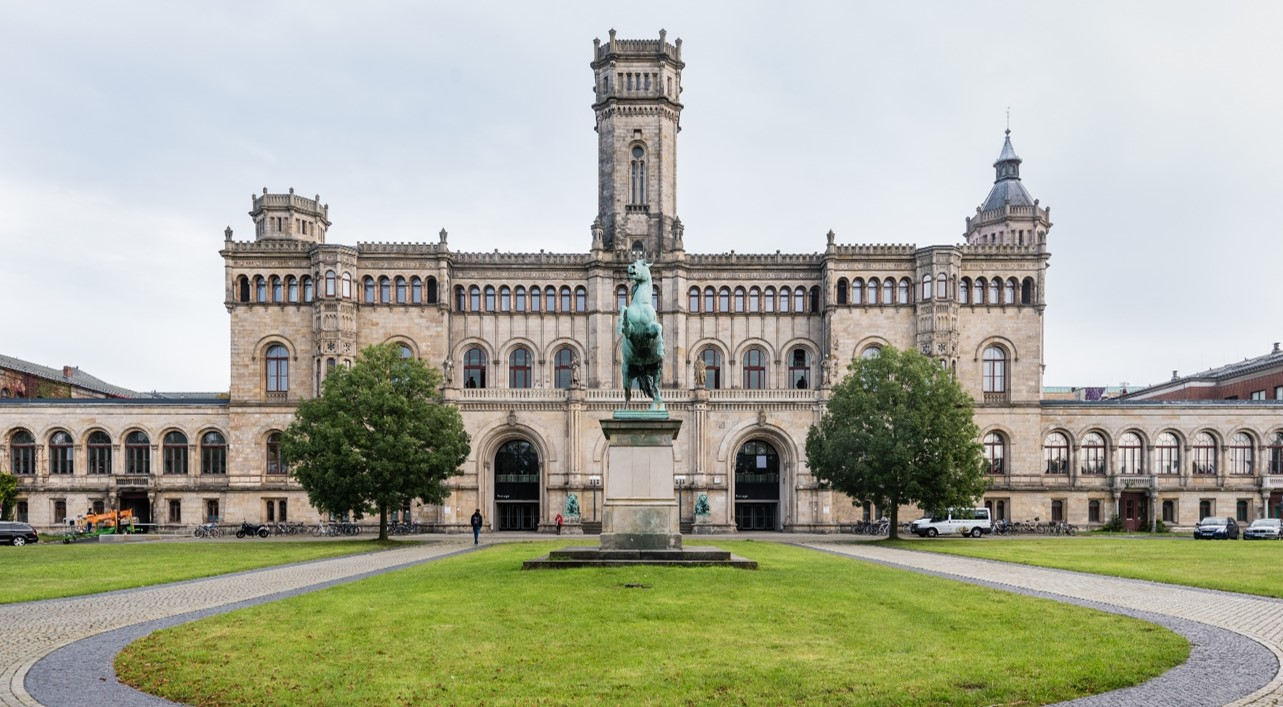
\includegraphics[width=0.65\textwidth]{figures/luh_default_presentation_title_image.jpg}}

% Title page: luhstyle
% \setbeamertemplate{title page}[luhstyle]
% % Add optional title image here
% \addtitlepageimage{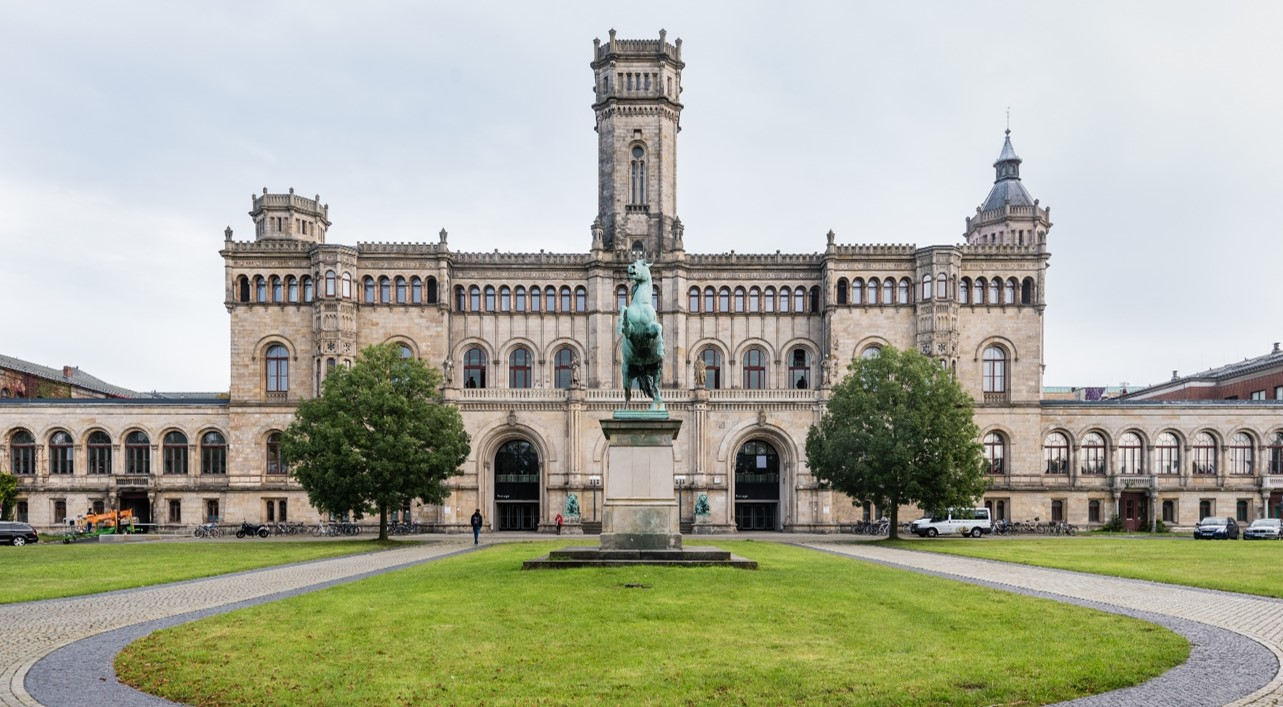
\includegraphics[width=0.75\textwidth]{figures/luh_default_presentation_title_image.jpg}}

\author[Abedjan \& Lindauer]{Ziawasch Abedjan \& Marius Lindauer\\[1em]
	
\includegraphics[height=\logoheight]{../latex_main/figures/luh_logo_rgb_0_80_155.pdf}\qquad
	
\includegraphics[height=\logoheight]{../latex_main/figures/DBIS_Kurzlogo.png}\qquad

\includegraphics[height=\logoheight]{../latex_main/figures/TNT_darkv4}\qquad

\includegraphics[height=\logoheight]{../latex_main/figures/L3S.jpg}	}
\date{Summer Term 2022; \hspace{0.5em} {
\includegraphics[height=1.5em]{../latex_main/figures/Cc-by-nc-sa_icon.svg.png}}; based on \href{https://ds100.org/fa21/}{[DS100]}
}


%%% Custom Packages
%----------------------------------------------------------------------
% Create dummy content
\usepackage{blindtext}

% Adds a frame with the current page layout. Just call \layout inside of a frame.
\usepackage{layout}


%%% Macros
%\renewcommand{\vec}[1]{\mathbf{#1}}
% \usepackage{bm}
%\let\vecb\bm

\title[Introduction]{DS: Decision Trees}
\subtitle{}

\graphicspath{ {./figure/} }
%\institute{}


\begin{document}
	
	\maketitle
	\begin{frame}{Decision Trees}
	    A Decision Tree is a very simple way to classify data. It is simply a tree of questions that must be answered in sequence to yield a predicted classification.
	    \begin{figure}
	        \centering
	        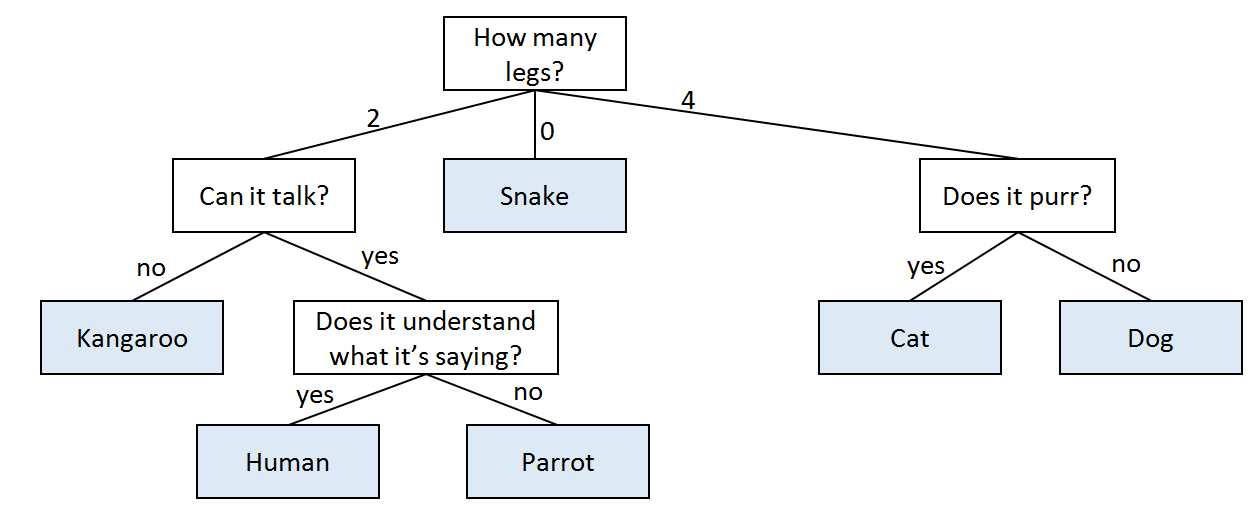
\includegraphics[scale=.35]{Bild1}
	    \end{figure}
	\end{frame}
	
	
	\begin{frame}{Example: Flower Classification}
	    The Iris flower data set is a commonly used example:
	    \begin{itemize}
	        \item Created by statistician/biologist Ronald Fisher for his paper “The use of multiple measurements in taxonomic problems”.
	        \item Data set consists of 150 flower measurements from 3 different species.
	        \item For each, we have “petal length”, “petal width”, “sepal length”, “sepal width”.
	    \end{itemize}
	    Goal is to predict species from other data.
	    \begin{figure}
	        \centering
	        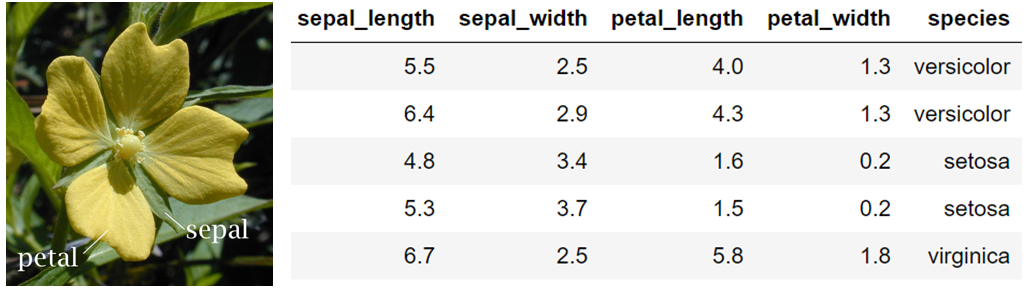
\includegraphics[scale=.35]{Bild2}
	    \end{figure}
	    \url{https://en.wikipedia.org/wiki/Sepal}

	\end{frame}
	
		\begin{frame}{Example: Logistic Regression Using Petal Data Only}
	    The plot below shows the width and length of the petals of each flower, with the species annotated in the form of color.
	    \begin{figure}
	        \centering
	        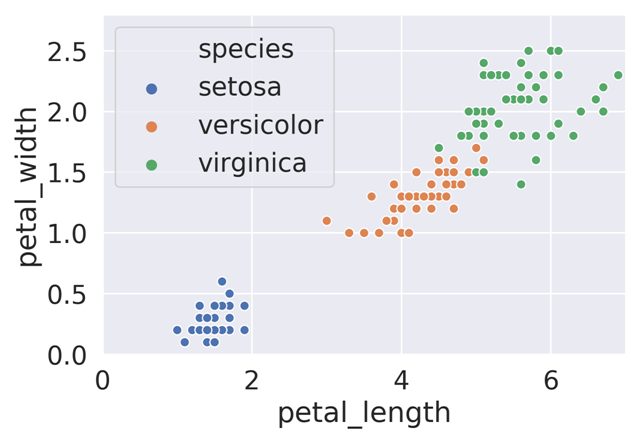
\includegraphics[scale=.75]{Bild3}
	    \end{figure}
	\end{frame}
	
	\begin{frame}{Example: Logistic Regression Using Petal Data Only}
	    The plot below shows the width and length of the petals of each flower, with the species annotated in the form of color.
	    \begin{itemize}
	        \item If we train a 3 class logistic regression model on this data, we end up with the model below.
	        \item See extra slides from lecture 19 for more details on how this works.
	    \end{itemize}
	    \begin{figure}
	        \centering
	        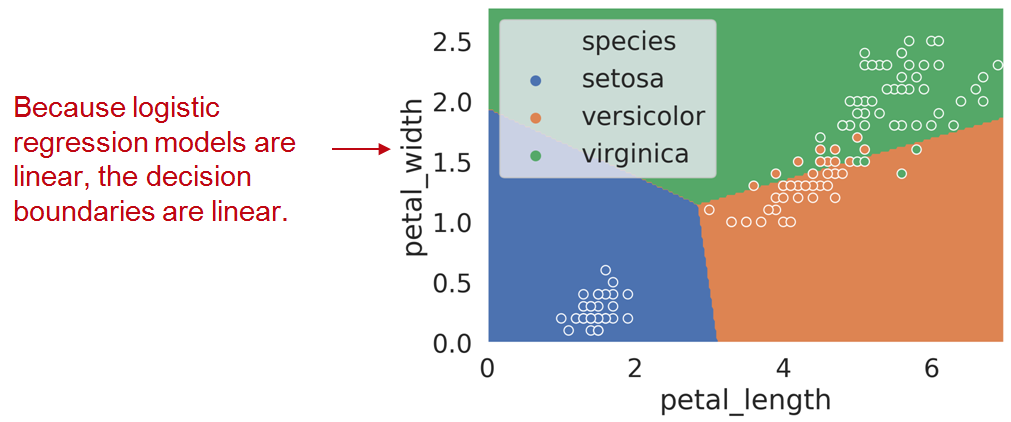
\includegraphics[scale=.4]{Bild4}
	    \end{figure}
	\end{frame}
	
	
	\begin{frame}{Example: Using Petal Data Only}
	    The plot below shows the width and length of the petals of each flower, with the species annotated in the form of color.\\
	    \bigskip
	    We can build a decision tree manually just by looking at this picture.
	    \begin{figure}
	        \centering
	        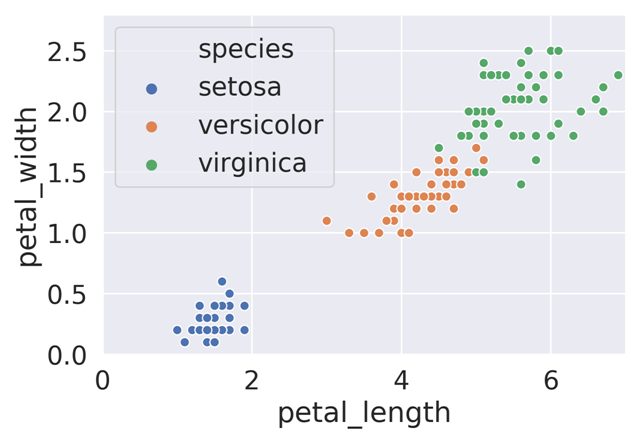
\includegraphics[scale=.65]{Bild3}
	    \end{figure}
	\end{frame}
	
	\begin{frame}{Example: Using Petal Data Only}
	    \begin{figure}
	        %\centering
	        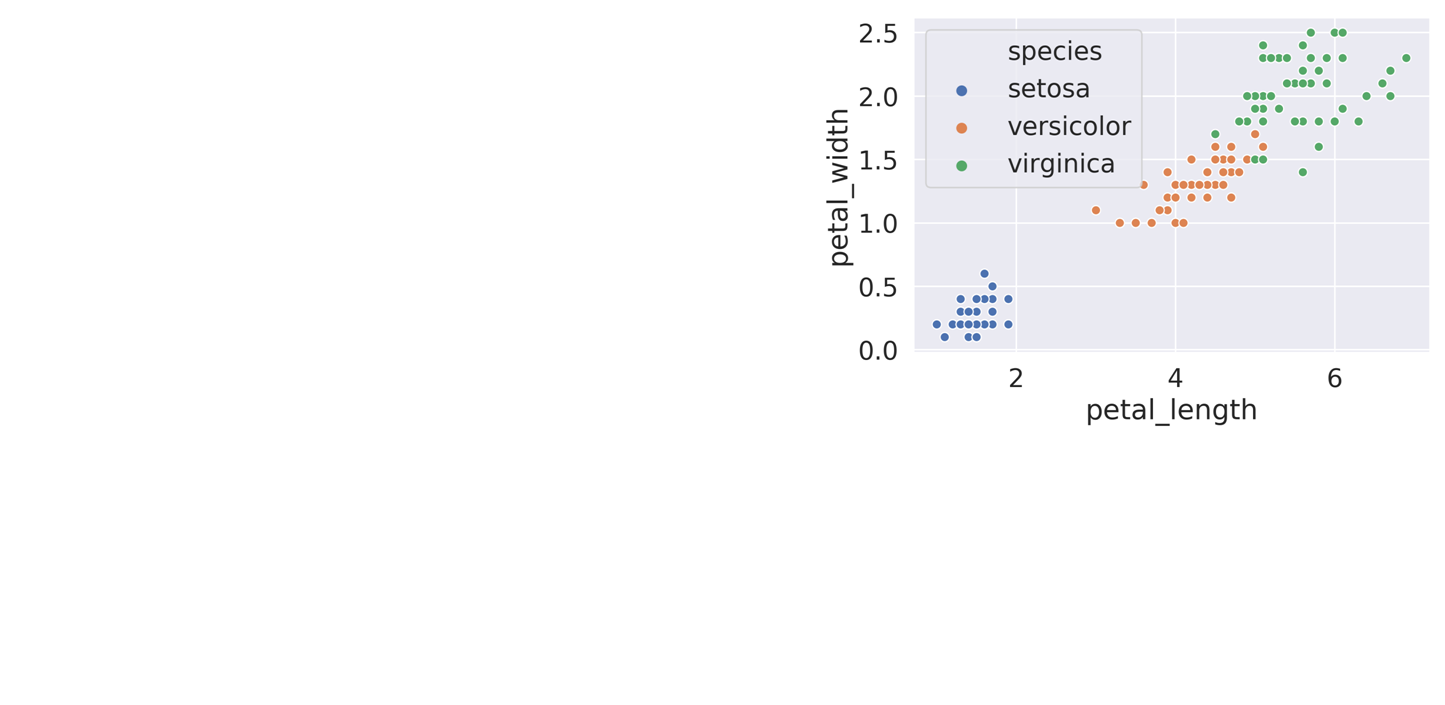
\includegraphics[scale=.34]{Bild5}
	    \end{figure}
	\end{frame}
	
	
	\begin{frame}{Example: Using Petal Data Only}
	    \begin{figure}
	        %\centering
	        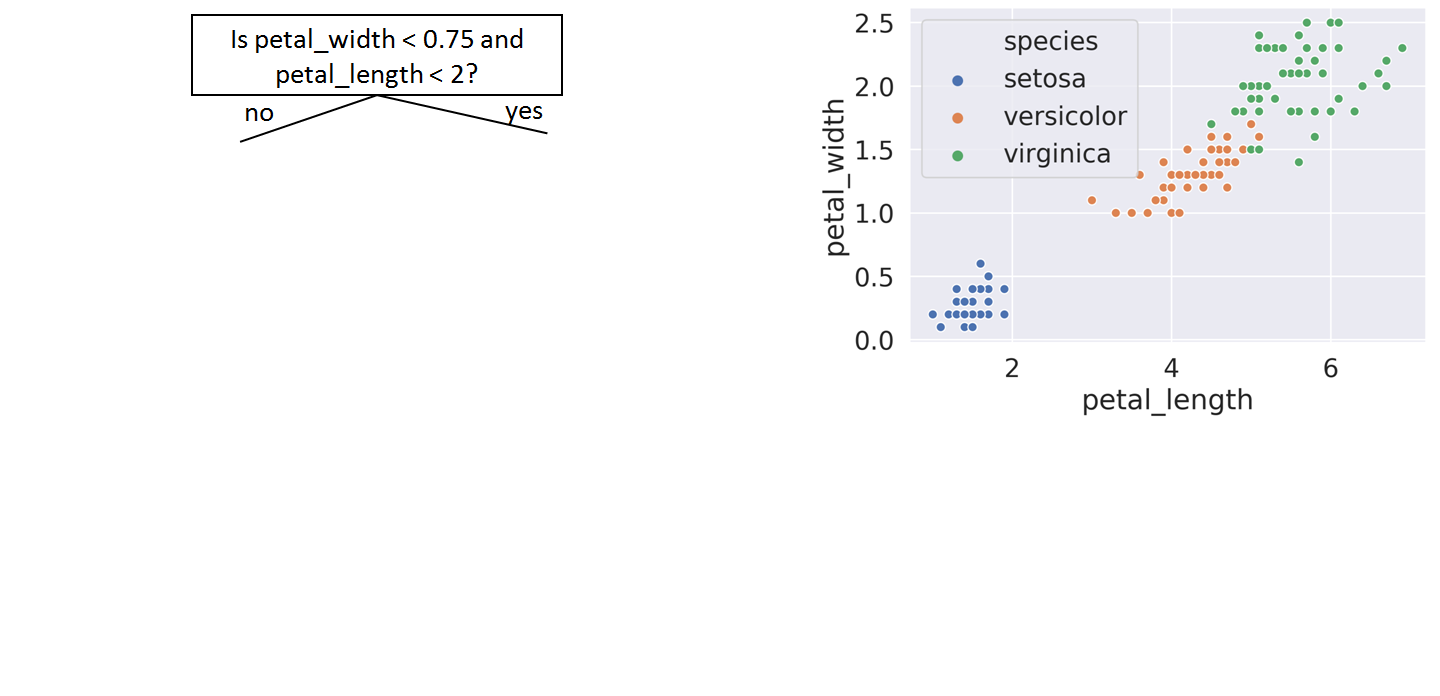
\includegraphics[scale=.34]{Bild6}
	    \end{figure}
	\end{frame}
	
	
	\begin{frame}{Example: Using Petal Data Only}
	    \begin{figure}
	        %\centering
	        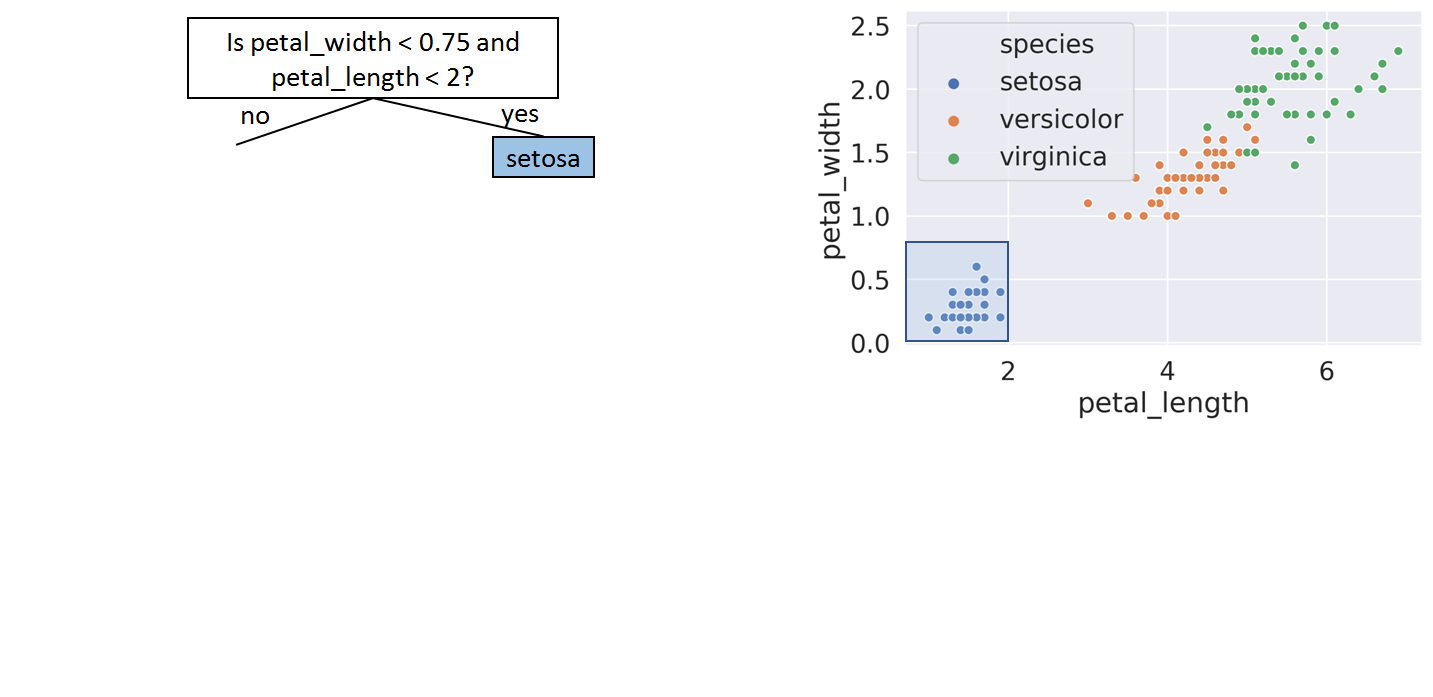
\includegraphics[scale=.34]{Bild7}
	    \end{figure}
	\end{frame}
	
	
	\begin{frame}{Example: Using Petal Data Only}
	    \begin{figure}
	        %\centering
	        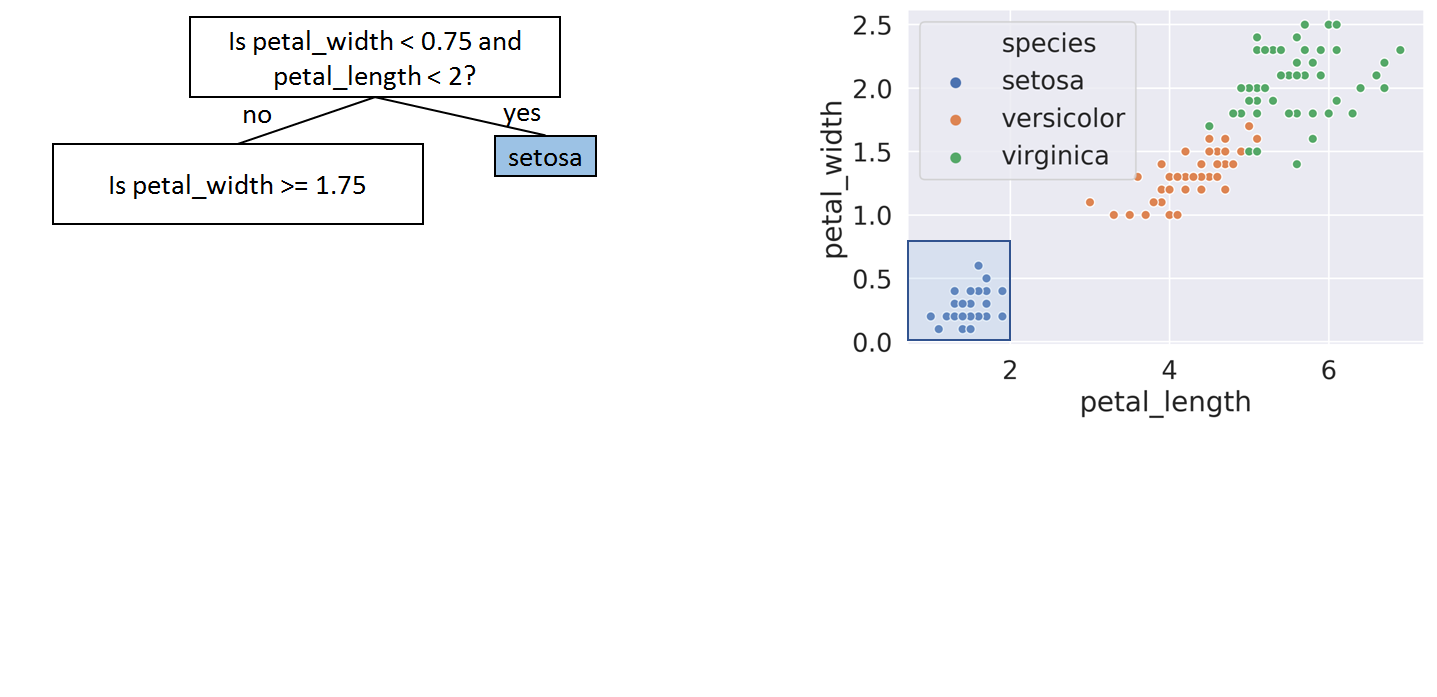
\includegraphics[scale=.34]{Bild8}
	    \end{figure}
	\end{frame}
	
	
	\begin{frame}{Example: Using Petal Data Only}
	    \begin{figure}
	        %\centering
	        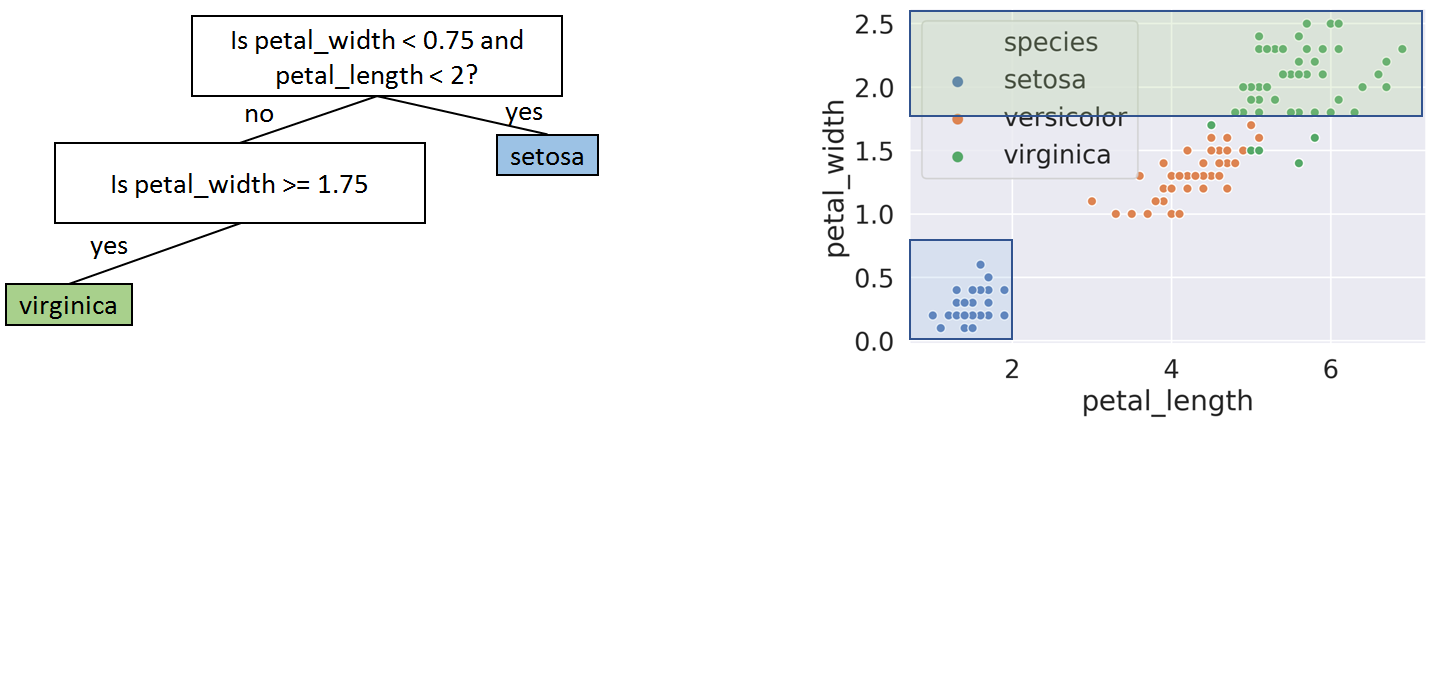
\includegraphics[scale=.34]{Bild9}
	    \end{figure}
	\end{frame}
	
	
	\begin{frame}{Example: Using Petal Data Only}
	    \begin{figure}
	        %\centering
	        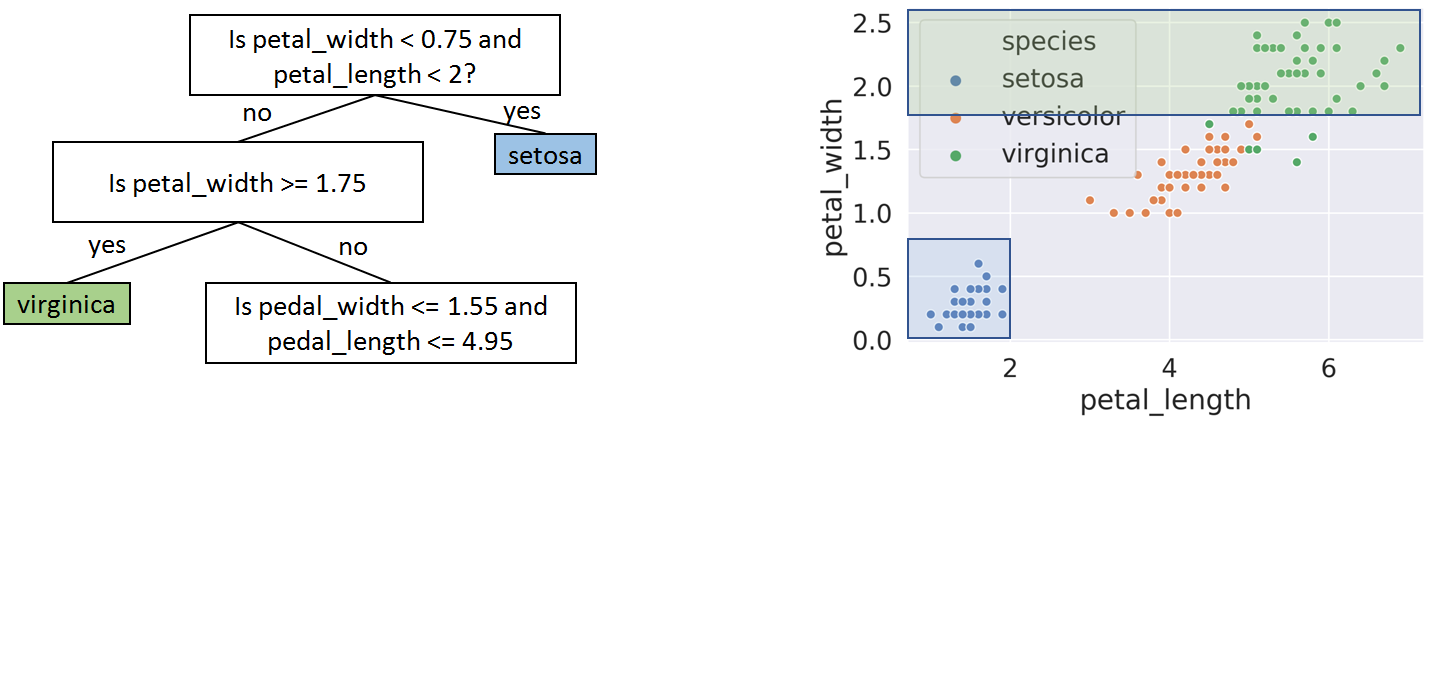
\includegraphics[scale=.34]{Bild10}
	    \end{figure}
	\end{frame}
	
	
	\begin{frame}{Example: Using Petal Data Only}
	    \begin{figure}
	        %\centering
	        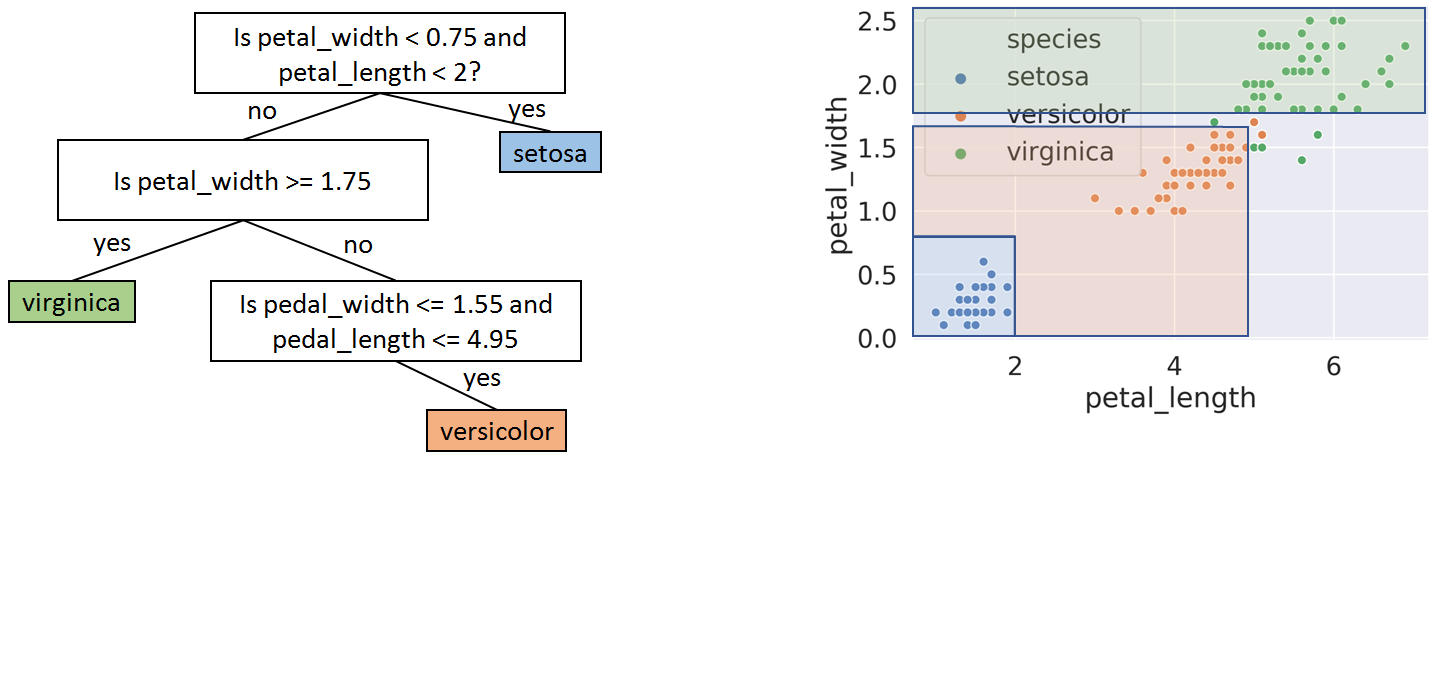
\includegraphics[scale=.34]{Bild11}
	    \end{figure}
	\end{frame}
	
	
	\begin{frame}{Example: Using Petal Data Only}
	    \begin{figure}
	        %\centering
	        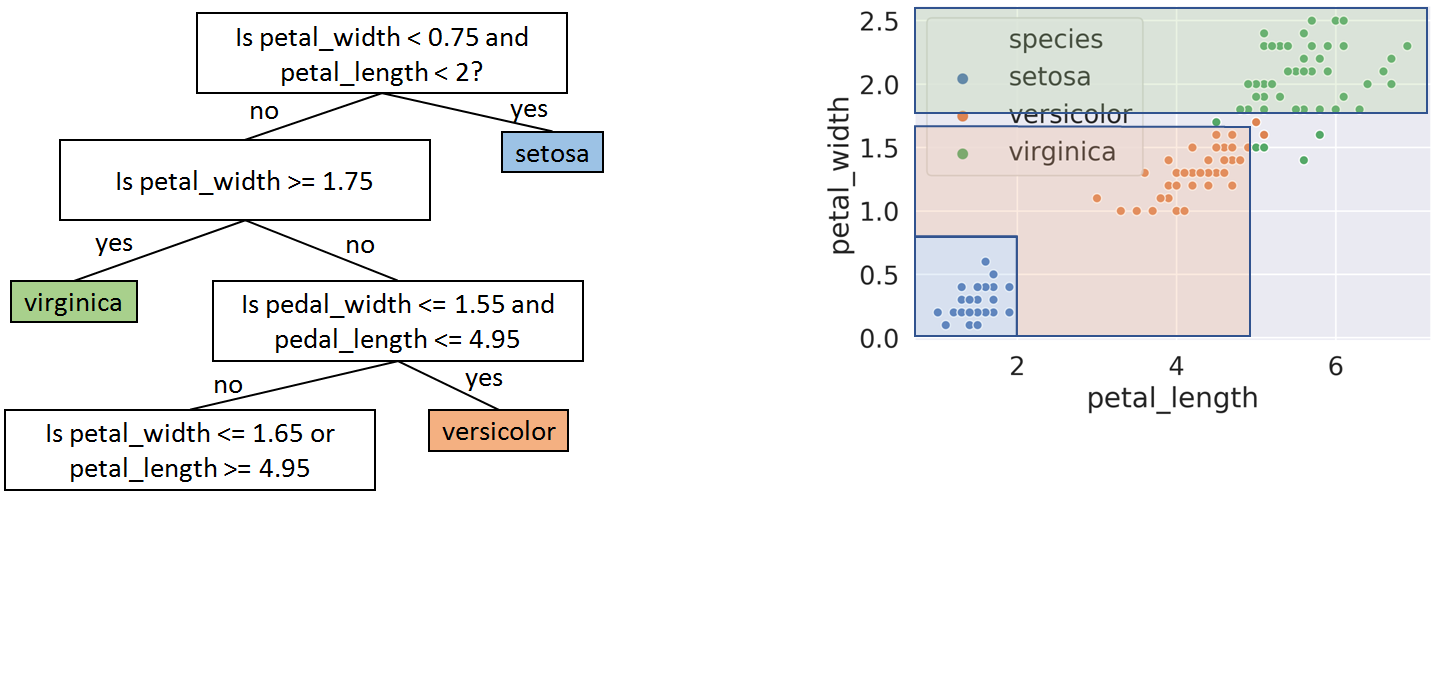
\includegraphics[scale=.34]{Bild12}
	    \end{figure}
	\end{frame}
	
	
	\begin{frame}{Example: Using Petal Data Only}
	    \begin{figure}
	        %\centering
	        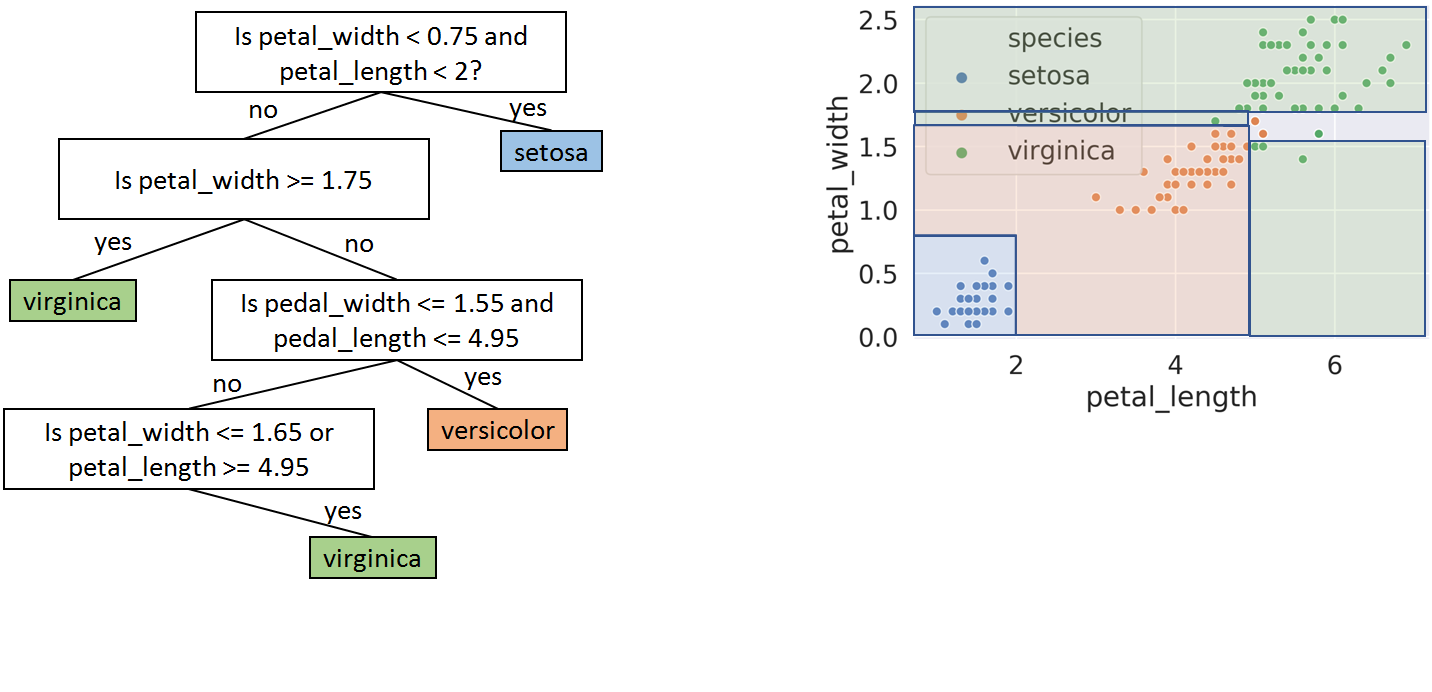
\includegraphics[scale=.34]{Bild13}
	    \end{figure}
	\end{frame}
	
	
	\begin{frame}{Example: Using Petal Data Only}
	    \begin{figure}
	        %\centering
	        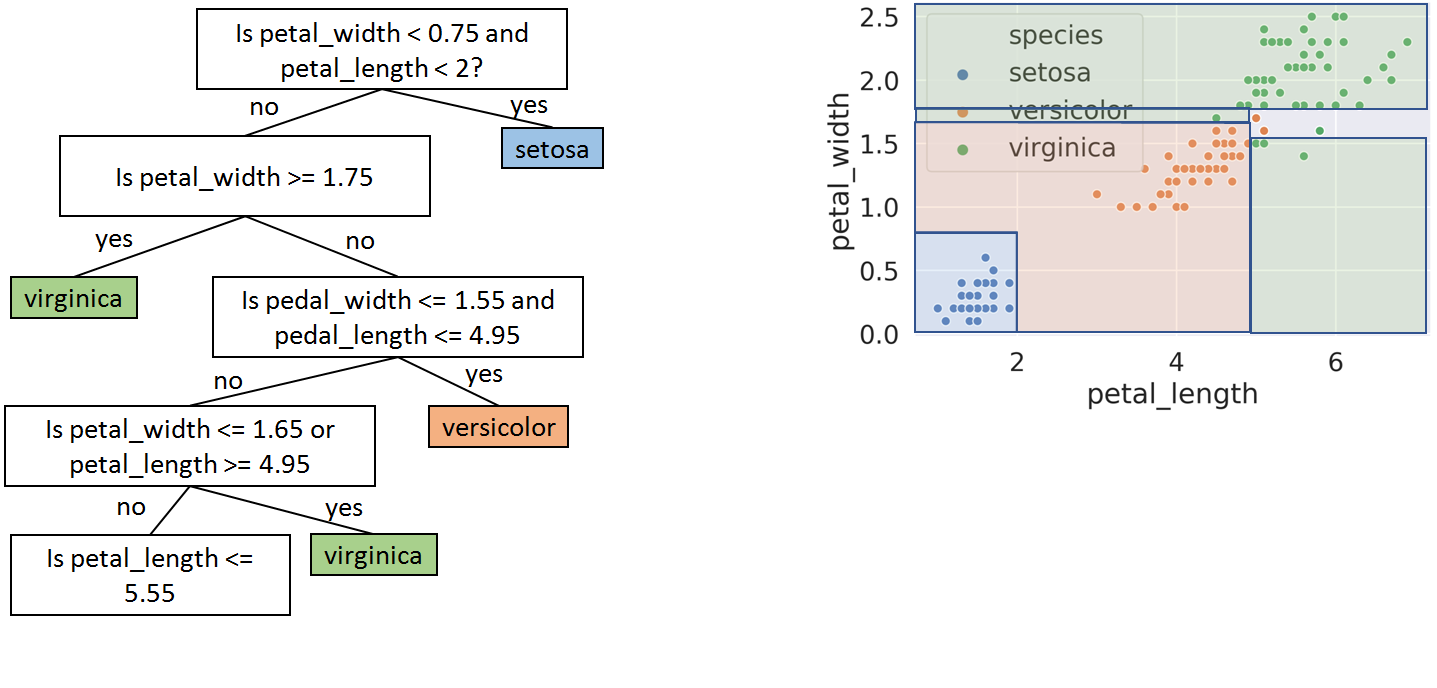
\includegraphics[scale=.34]{Bild14}
	    \end{figure}
	\end{frame}
	
	
	\begin{frame}{Example: Using Petal Data Only}
	    \begin{figure}
	        %\centering
	        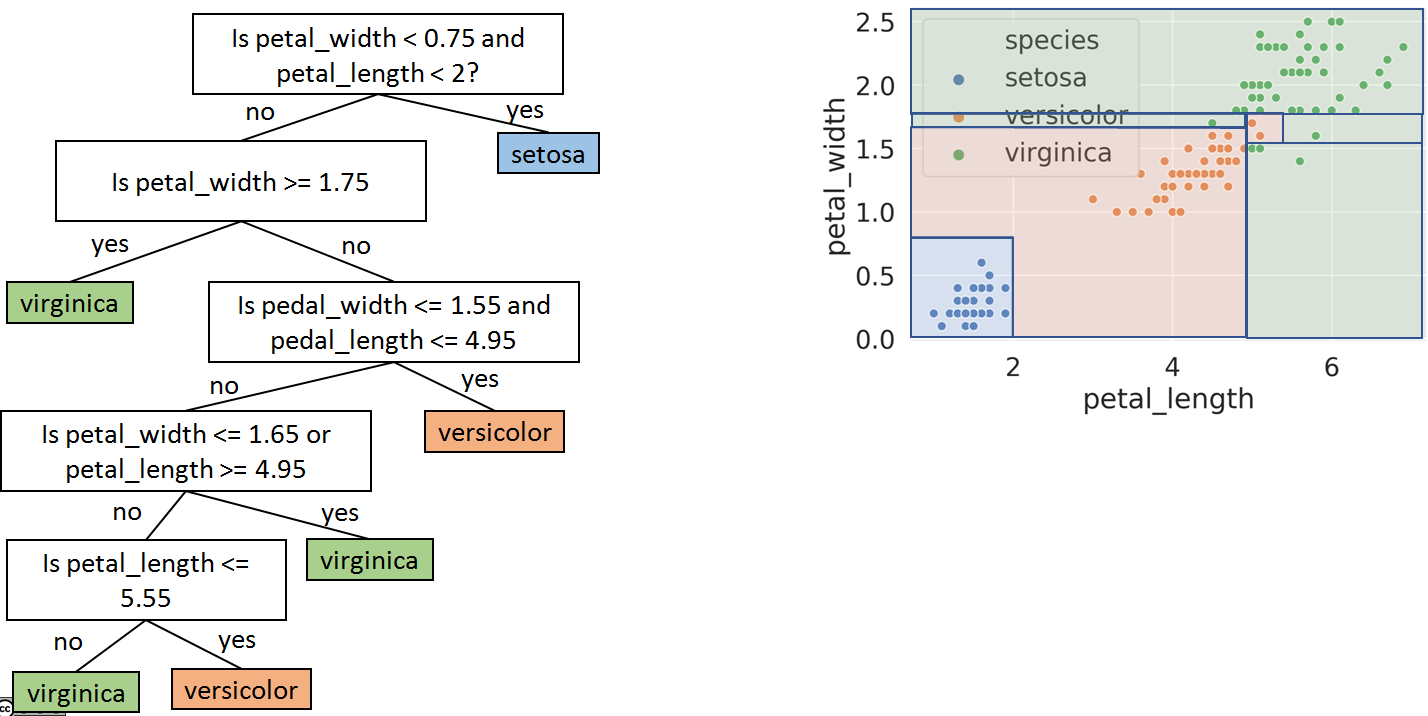
\includegraphics[scale=.34]{Bild15}
	    \end{figure}
	\end{frame}
	
	
	\begin{frame}{Example: Using Petal Data Only}
	   \begin{columns}
	        \begin{column}{.5\textwidth}
	               How accurate is our decision tree model on the training data?\\
	               \bigskip
	                Is this good or bad?
	        \end{column}
	   
	   
	         \begin{column}{.5\textwidth}
	               \begin{figure}
	                    %\centering
	                     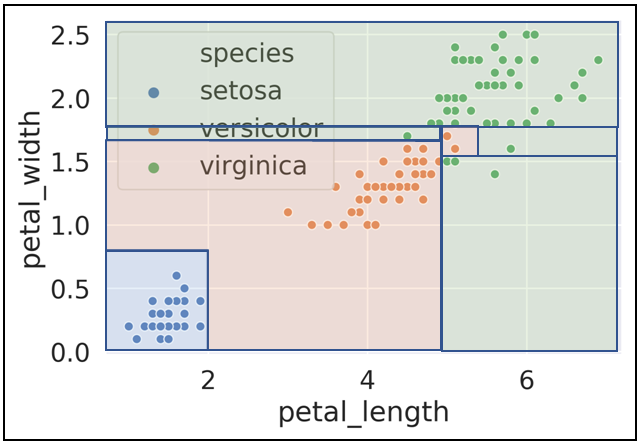
\includegraphics[scale=.34]{Bild16}
	                \end{figure}
	        \end{column}
	   \end{columns}
	 \end{frame}
	 
	 
	 \begin{frame}{Example: Using Petal Data Only}
	   \begin{columns}
	        \begin{column}{.5\textwidth}
	               How accurate is our decision tree model on the training data?\\
	               \begin{itemize}
	                   \item It seems like it gets every point correct
	               \end{itemize}
	               \bigskip
	                Is this good or bad?
	                \begin{itemize}
	                    \item I’d argue bad
	                    \item Seems likely to result in overfitting!
	                    \item Will discuss overfitting more later
	                \end{itemize}
	                First, let’s see how we can build decision trees for classification using scikit-learn
	        \end{column}
	   
	   
	         \begin{column}{.5\textwidth}
	               \begin{figure}
	                    %\centering
	                     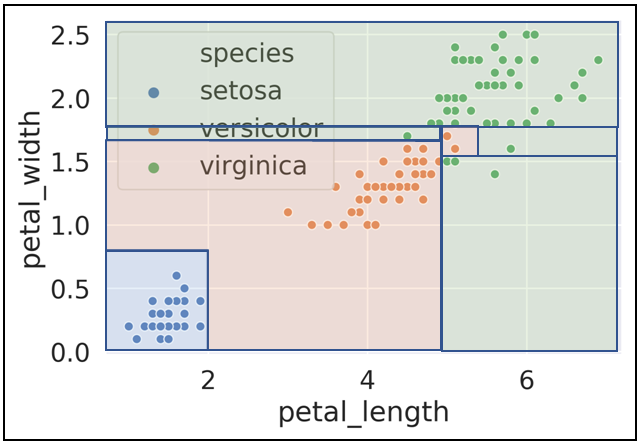
\includegraphics[scale=.34]{Bild16}
	                \end{figure}
	        \end{column}
	   \end{columns}
	 \end{frame}
	
	
		\begin{frame}{Decision Tree Models With scikit-learn }
	    The code to build a decision tree model in scikit-learn is very similar to what we saw for building linear and logistic regression models:
	    \begin{figure}
	        \centering
	        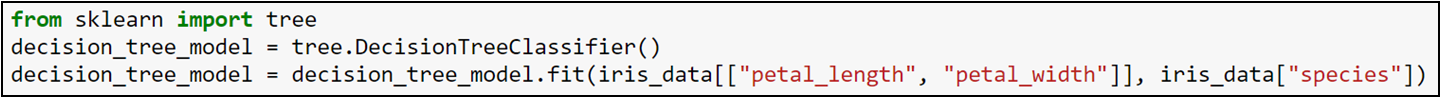
\includegraphics[scale=.6]{Bild17}
	    \end{figure}
	    See lec20-decision-trees.ipynb if you want to try it out
	\end{frame}
	
	
	
	\begin{frame}{Decision Tree Models With scikit-learn }
	    The code to build a decision tree model in scikit-learn is very similar to what we saw for building linear and logistic regression models:
	    \begin{figure}
	        \centering
	        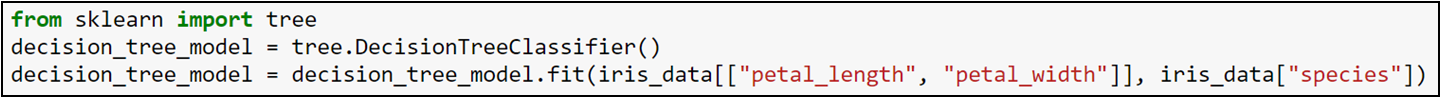
\includegraphics[scale=.6]{Bild17}
	    \end{figure}
	    See lec20-decision-trees.ipynb if you want to try it out
        \begin{figure}
            \centering
            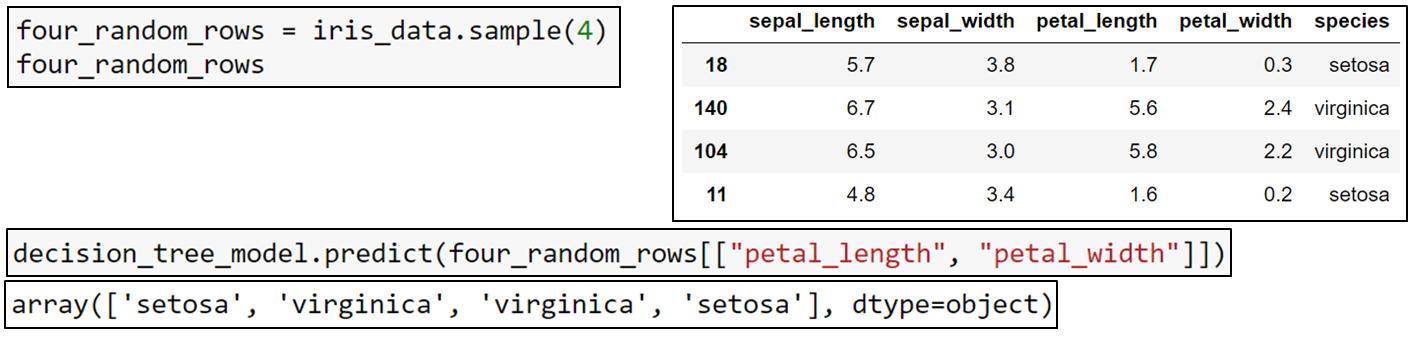
\includegraphics[scale=.4]{Bild18}
        \end{figure}
	\end{frame}
	
	
	\begin{frame}{Visualizing Decision Tree Models }
	    \begin{figure}
	        \centering
	        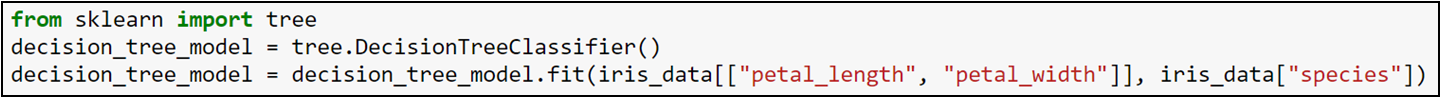
\includegraphics[scale=.6]{Bild17}
	    \end{figure}
	    Suppose we want to visualize the decision tree, similar to what we saw earlier:
        \begin{figure}
            \centering
            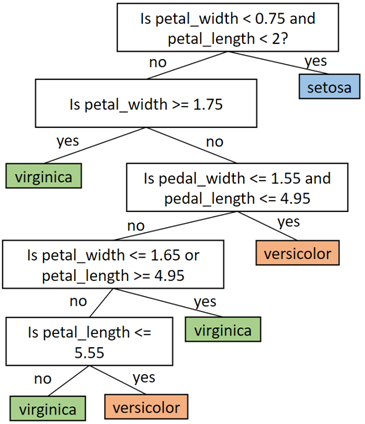
\includegraphics[scale=.65]{Bild19}
        \end{figure}
	\end{frame}
	
	
	\begin{frame}{Visualizing Decision Tree Models }
	    \begin{figure}
	        \centering
	        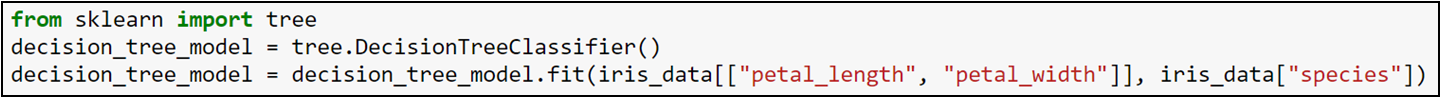
\includegraphics[scale=.6]{Bild17}
	    \end{figure}
	    \begin{columns}
	        \begin{column}{.5\textwidth}
	                \begin{figure}
	                    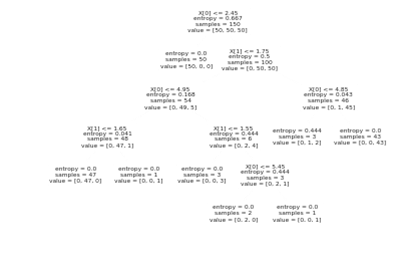
\includegraphics[scale=.55]{Bild22}
	                \end{figure}
	        \end{column}
	        
	        
	        \begin{column}{.5\textwidth}
	                There is a built in DecisionTree visualizer
	                \begin{itemize}
	                    \item Unfortunately, it isn’t very good
	                \end{itemize}
	                \begin{figure}
	                    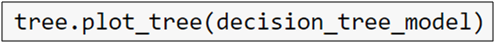
\includegraphics[scale=.65]{Bild21}
	                \end{figure}
	        \end{column}
	    \end{columns}
	\end{frame}
	
	
	\begin{frame}{Visualizing Decision Tree Models }
	    \begin{columns}
	        \begin{column}{.4\textwidth}
	        Can use GraphViz to get a much nicer picture.
	                \begin{figure}
	                    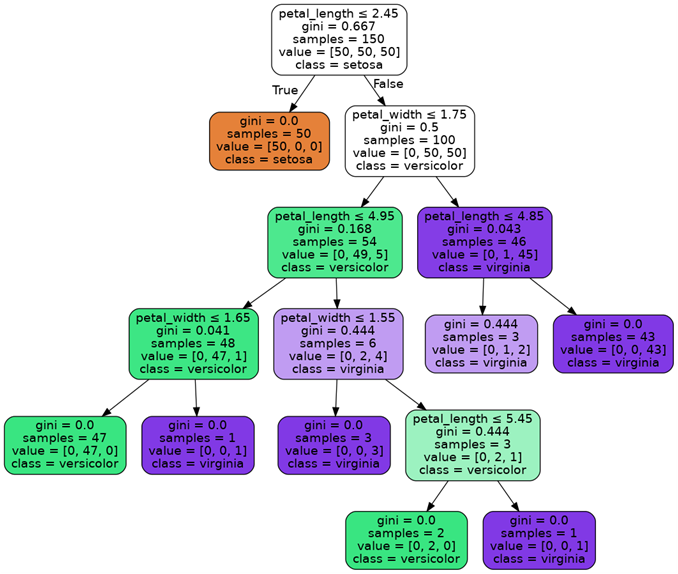
\includegraphics[scale=.5]{Bild23}
	                \end{figure}
	        \end{column}
	        
	        
	        \begin{column}{.6\textwidth}
	                \begin{figure}
	                    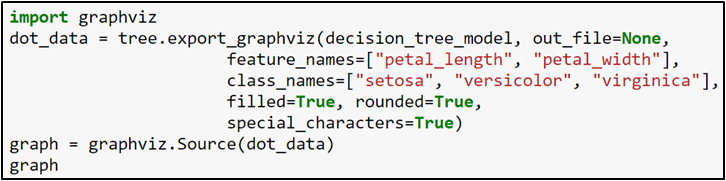
\includegraphics[scale=.55]{Bild24}
	                \end{figure}
	                In each box, we see:
	                \begin{itemize}
	                    \item The rule
	                    \item The gini impurity (chance that a sample would be misclassified if randomly assigned at this point)
	                    \item The number of samples still unclassified
	                    \item The number of samples in each class still unclassified
	                    \item The most likely class
	                \end{itemize}
	        \end{column}
	    \end{columns}
	\end{frame}
	
	
	\begin{frame}{Visualizing Decision Tree Models }
	    \begin{columns}
	        \begin{column}{.4\textwidth}
	        Can use GraphViz to get a much nicer picture.
	                \begin{figure}
	                    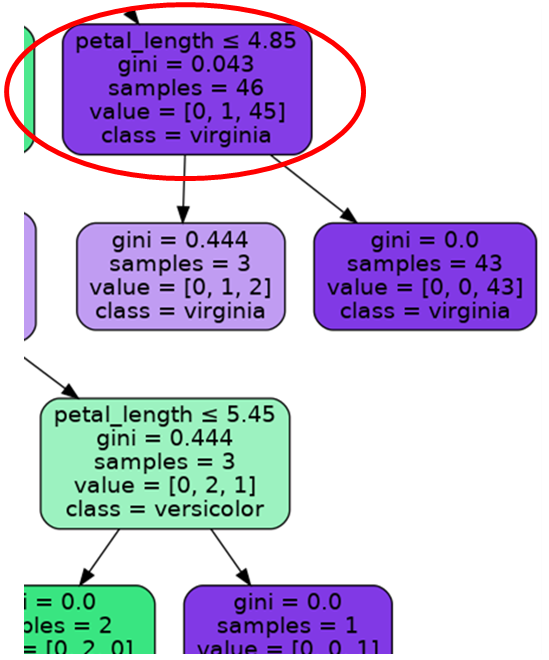
\includegraphics[scale=.3]{Bild25}
	                \end{figure}
	        \end{column}
	        
	        
	        \begin{column}{.6\textwidth}
	                \begin{figure}
	                    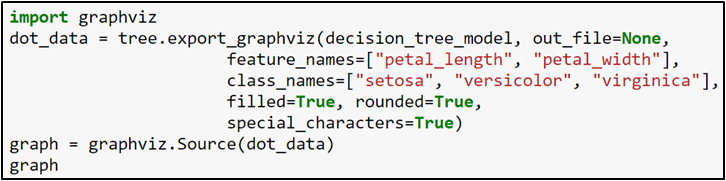
\includegraphics[scale=.55]{Bild24}
	                \end{figure}
	                In each box, we see:
	                \begin{itemize}
	                    \item The rule
	                    \item The gini impurity (chance that a sample would be misclassified if randomly assigned at this point)
	                    \item The number of samples still unclassified
	                    \item The number of samples in each class still unclassified
	                    \item The most likely class
	                \end{itemize}
	        \end{column}
	    \end{columns}
	\end{frame}
	
	
	\begin{frame}{Visualizing Decision Tree Models}
	    Plotting the decision boundaries for our logistic regression & decision tree models, yields these results:
	    \begin{itemize}
	        \item Decision tree has nonlinear boundary, and appears to get 100\% accuracy
	        \begin{itemize}
	            \item Let’s calculate the exact accuracy rather than just relying on our eyes
	        \end{itemize}
	    \end{itemize}
	    \begin{figure}
	        \centering
	        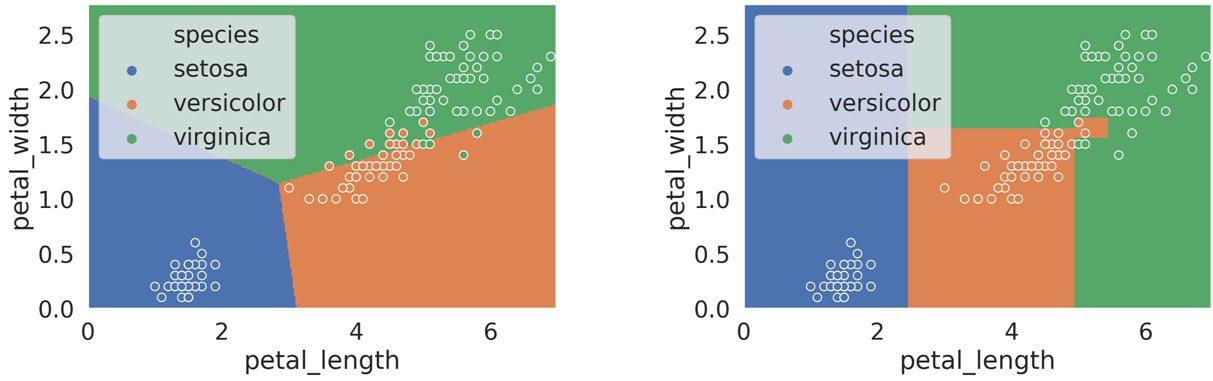
\includegraphics[scale=.45]{Bild26}
	    \end{figure}
	\end{frame}
	
	
	\begin{frame}{Measuring the Performance of Our Model}
	    Running the code below, we see that we only get 99.3% accuracy
        \begin{figure}
            \centering
            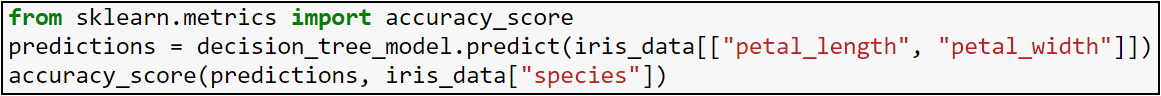
\includegraphics[scale=.65]{Bild27}
        \end{figure}
        To understand why, let’s look back at our decision tree model
	\end{frame}
	
	
	\begin{frame}{Understanding Our Decision Tree}
	    \begin{columns}
	        \begin{column}{.5\textwidth}
	                \begin{figure}
	                    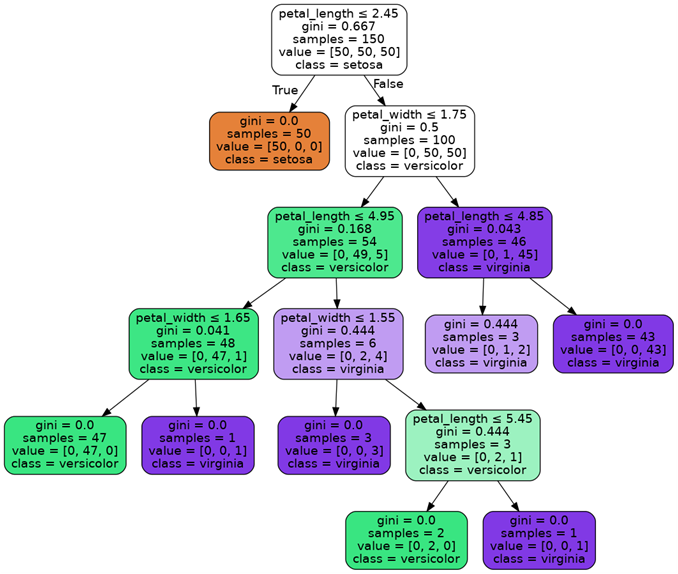
\includegraphics[scale=.55]{Bild23}
	                \end{figure}
	        \end{column}
	        
	        
	         \begin{column}{.5\textwidth}
	                \\ \bigskip \bigskip
	                There is one terminal decision point where there is more than one possible right answer\\
	                \bigskip
	                Can you find it?
	        \end{column}
	    \end{columns}
	\end{frame}
	
	
	
	
	\begin{frame}{Understanding Our Decision Tree}
	    \begin{columns}
	        \begin{column}{.5\textwidth}
	                \begin{figure}
	                    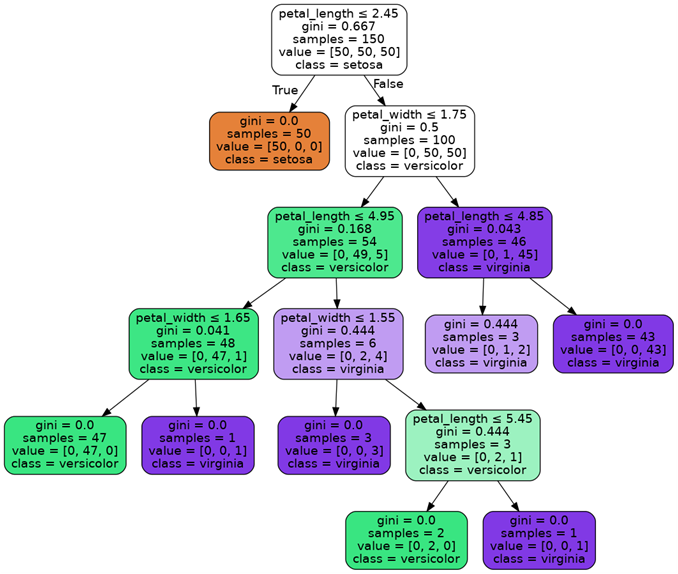
\includegraphics[scale=.55]{Bild23}
	                \end{figure}
	        \end{column}
	        
	        
	         \begin{column}{.5\textwidth}
	                \\ \bigskip \bigskip
	                There is one terminal decision point where there is more than one possible right answer\\
	                \bigskip
	                The model was unable to come up with a decision rule to resolve these last 3 samples\\
	                \bigskip
	                Let’s see why using the query method of the dataframe class
	        \end{column}
	    \end{columns}
	\end{frame}
	
	
	\begin{frame}{Understanding Our Decision Tree}
	                \begin{figure}
	                    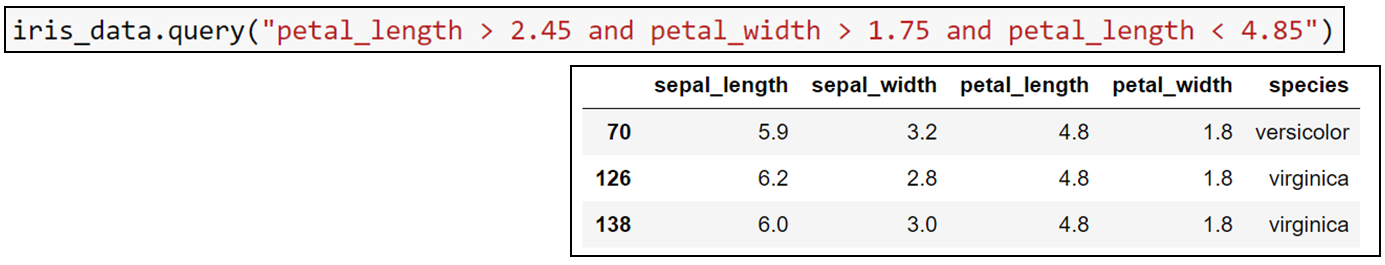
\includegraphics[scale=.3]{Bild28}
	                \end{figure}
	    \begin{columns}
	        \begin{column}{.4\textwidth}
	                \begin{figure}
	                    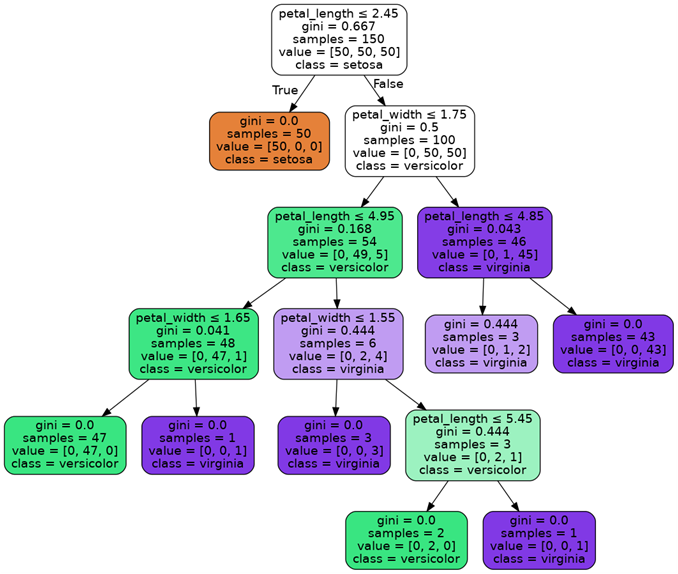
\includegraphics[scale=.35]{Bild23}
	                \end{figure}
	        \end{column}
	        
	        
	         \begin{column}{.4\textwidth}
	                There is one terminal decision point where there is more than one possible right answer
	                \begin{itemize}
	                    \item In the original data set, there was a versicolor iris with the same petal measurements as two virginicas
	                \end{itemize}
	        \end{column}
	    \end{columns}
	\end{frame}
	
	
	
	\begin{frame}{Overfitting and Decision Trees}
	    Bottom line: scikit-learn makes it easy to generate decision trees
	    \begin{figure}
	        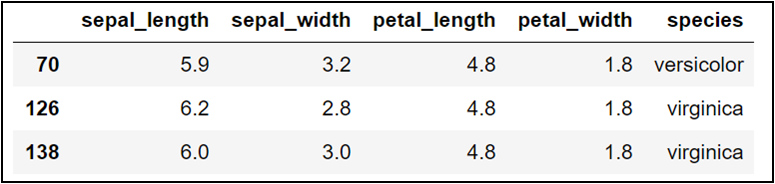
\includegraphics[scale=.5]{Bild29}
	    \end{figure}
	    These decision trees will always have perfect accuracy on the training data, EXCEPT when there are samples from different categories with the exact same features
	    \begin{itemize}
	        \item That is, if the versicolor above had a petal\_length of 4.800001, we’d have 100\% training accuracy
	    \end{itemize}
	    \\
	    \bigskip
	    This tendency for perfect accuracy should give us concern about overfitting
	\end{frame}
	
	
		\begin{frame}{Overfitting and Decision Trees}
	    With the exception of samples that have the exact same data, we can always get 100\% accuracy. This should give us concern about possible overfitting\\
	    \bigskip
	    Let’s see how bad things are by separating our data into train and test sets
	    \begin{itemize}
	        \item We’ll use 110 training points and 40 testing points
	        \item Performance on test set gives us an estimate of how well we generalize
	    \end{itemize}
	    \begin{figure}
	        \centering
	        \includegraphics[scale=.4]{Bild30}
	    \end{figure}
	\end{frame}
	
	\begin{frame}{Visualizing Our New Model}
	   Comparing our model trained on 150 vs. 110 data points, we see slight differences in the generated model\\
	    \begin{itemize}
	        \item Naturally, both models get very high accuracy on the data that they use for training (100\% for non-overlapping points)
	    \end{itemize}
	    \begin{figure}
	        \centering
	        \includegraphics[scale=.4]{Bild31}
	    \end{figure}
	\end{frame}
	
	
	\begin{frame}{Performance of Our New Model on the Test Set}
	  When we look at the performance of Model 2D-110 on the test set, we see that we make some errors that aren’t just from overlapping data\\
	    \begin{itemize}
	        \item 99\% accuracy on training set (2 overlapping points). 95\% accuracy on test set
	    \end{itemize}
	    \begin{figure}
	        \centering
	        \includegraphics[scale=.4]{Bild31}
	    \end{figure}
	\end{frame}
	
	
	\begin{frame}{Multidimensional Decision Trees}
	  Naturally, we can include even more features. For example, if we want to use the petal AND sepal measurements, we simply train the decision tree on all four columns of the data\\
	  \begin{figure}
	        \centering
	        \includegraphics[scale=.6]{Bild32}
	    \end{figure}
	    The resulting model Model 4D-110 gets:
	    \begin{itemize}
	        \item 100\% accuracy on the training set (no overlapping data points)
            \item 95\% accuracy on the test set
	    \end{itemize}
	    Cannot easily visualize Model 4D-110’s decision   boundaries because the prediction space   is 4 dimensional
	\end{frame}
	
	
	\begin{frame}{Model 2D-150 vs. Model 4D-110 Tree Visualization}
	    \begin{columns}
	        \begin{column}{.5\textwidth}
	                \begin{figure}
	                    \includegraphics[scale=.53]{Bild23}
	                \end{figure}
	        \end{column}
	   
	        \begin{column}{.5\textwidth}
	                \begin{figure}
	                    \includegraphics[scale=.33]{Bild35}
	                \end{figure}
	        \end{column}
	    \end{columns}
	    What is different about these two models?
	\end{frame}
	
	
	\begin{frame}{Model 2D-150 vs. Model 4D-110 Tree Visualization}
	    \begin{columns}
	        \begin{column}{.5\textwidth}
	                Models are quite similar:
	                \begin{itemize}
	                    \item Model 4D-110 uses only 110 samples.
	                    \item The decision rules are nearly identical, except that Model4D-110 uses the sepal\_width exactly once to resolve the case that we couldn’t resolve with petal\_length and petal\_width
	                \end{itemize}
	                Model 4D-110 seems marginally better to me, but both got only 95\% accuracy on test set. 
	                \begin{itemize}
	                    \item Need more data to know for sure
	                \end{itemize}
	        \end{column}
	   
	        \begin{column}{.5\textwidth}
	                \begin{figure}
	                    \includegraphics[scale=.33]{Bild35}
	                \end{figure}
	        \end{column}
	    \end{columns}
	 
	\end{frame}
	
	
	
	\begin{frame}{Model 2D-150 vs. Model 4D-110 Tree Visualization}
	    \begin{columns}
	        \begin{column}{.5\textwidth}
	                Models are quite similar:
	                \begin{itemize}
	                    \item Model 4D-110 uses only 110 samples.
	                    \item The decision rules are nearly identical, except that Model4D-110 uses the sepal\_width exactly once to resolve the case that we couldn’t resolve with petal\_length and petal\_width
	                \end{itemize}
	                Model 4D-110 seems marginally better to me, but both got only 95\% accuracy on test set. 
	                \begin{itemize}
	                    \item Need more data to know for sure
	                \end{itemize}
	        \end{column}
	   
	        \begin{column}{.5\textwidth}
	                \begin{figure}
	                    \includegraphics[scale=.33]{Bild34}
	                \end{figure}
	        \end{column}
	    \end{columns}
	 
	\end{frame}
	
	
	\begin{frame}{Overfitting and Sepal Data}
	    If we use the sepal data only (no petal data), we will run into serious overfitting issues\\
	    \bigskip
	    Below, we see our three flowers plotted in the sepal space
	    \begin{figure}
	        \centering
	        \includegraphics[scale=.65]{Bild36}
	    \end{figure}
	\end{frame}
	
	
	\begin{frame}{Sepal Decision Boundaries}
	    After training on 110/150 points, we get the decision boundaries below
	    \begin{itemize}
	        \item Decision boundaries are erratic!
	        \item Many overlapping points leads to only 93\% accuracy on training set
	    \end{itemize}
	    \begin{figure}
	        \centering
	        \includegraphics[scale=.65]{Bild37}
	    \end{figure}
	\end{frame}
	
	
	
	\begin{frame}{Sepal Decision Boundaries and Test Set}
	    Performance on test set is quite poor
	    \begin{itemize}
	        \item Only 70\% accuracy: 28/40 predictions are correct
	    \end{itemize}
	    \begin{figure}
	        \centering
	        \includegraphics[scale=.65]{Bild38}
	    \end{figure}
	\end{frame}
	
	
	\begin{frame}{Overfitting Visualized}
	    The decision boundaries for our sepal model were quite complex
	    \begin{itemize}
	        \item Or drawn out as a tree, we also see a highly complex structure
	    \end{itemize}
	    Next, we’ll discuss strategies for preventing overfitting
	    \begin{figure}
	        \centering
	        \includegraphics[scale=.5]{Bild39}
	    \end{figure}
	\end{frame}
	
	
		\begin{frame}{Basic Decision Tree Generation}
	    \begin{figure}
	        \centering
	        \includegraphics[scale=.3]{Bild40}
	    \end{figure}
	\end{frame}
	
	\begin{frame}{Decision Tree Generation}
	    In order to understand how to avoid overfitting, let’s first discuss how decision trees are created from data\\
	    \bigskip
	    Traditional decision tree generation algorithm: 
	    \begin{itemize}
	        \item All of the data starts in the root node
	        \item Repeat until every node is either pure or unsplittable:
	        \begin{itemize}
	            \item Pick the best feature x and best split value $\beta$, e.g. x = petal\_length, $\beta$ = 2
	            \item Split data into two nodes, one where x < $\beta$, and one where x ≥ $\beta$
	        \end{itemize}
	    \end{itemize}
	    
	    
Notes: A node that has only one type is called a “pure” node. A node that has duplicate data that cannot be split is called “unsplittable”.

	\end{frame}
	
	
	\begin{frame}{Defining a Best Feature}
	    Question: Which feature and split value is best?
	    \begin{itemize}
	        \item  Equivalently: Which horizontal or vertical line do we want to draw?
	    \end{itemize}
	    \begin{figure}
	        \centering
	        \includegraphics[scale=.4]{Bild41}
	    \end{figure}
	\end{frame}
	
	\begin{frame}{Defining a Best Feature}
	    Question: Which feature and split value is best?
	    \begin{itemize}
	        \item  Equivalently: Which horizontal or vertical line do we want to draw?
	    \end{itemize}
	    \begin{figure}
	        \centering
	        \includegraphics[scale=.4]{Bild42}
	    \end{figure}
	\end{frame}
	
	\begin{frame}{Defining a Best Feature}
	    Question: Which feature and split value is best?
	    \begin{itemize}
	        \item  Equivalently: Which horizontal or vertical line do we want to draw?
	    \end{itemize}
	    \begin{figure}
	        \centering
	        \includegraphics[scale=.4]{Bild43}
	    \end{figure}
	\end{frame}
	
	\begin{frame}{Defining a Best Feature}
	    Question: Which feature and split value is best?
	    \begin{itemize}
	        \item  Equivalently: Which horizontal or vertical line do we want to draw?
	    \end{itemize}
	    \begin{figure}
	        \centering
	        \includegraphics[scale=.4]{Bild44}
	    \end{figure}
	\end{frame}
	
	\begin{frame}{Defining a Best Feature}
	    Question: Which feature and split value is best?
	    \begin{itemize}
	        \item  Equivalently: Which horizontal or vertical line do we want to draw?
	    \end{itemize}
	    \begin{figure}
	        \centering
	        \includegraphics[scale=.4]{Bild45}
	    \end{figure}
	\end{frame}
	
	
	\begin{frame}{Defining a Best Feature}
	    Question: Which feature and split value is best?
	    \begin{itemize}
	        \item  Equivalently: Which horizontal or vertical line do we want to draw?
	    \end{itemize}
	    We need some sort of rigorous definition for a good split
	    \begin{figure}
	        \centering
	        \includegraphics[scale=.4]{Bild45}
	    \end{figure}
	\end{frame}
	
	
	\begin{frame}{Defining a Best Feature}
	    Question: Which feature and split value is best?
	    \begin{itemize}
	        \item  Equivalently: Which horizontal or vertical line do we want to draw?
	    \end{itemize}
	    We need some sort of rigorous definition for a good split
	    \begin{figure}
	        \centering
	        \includegraphics[scale=.4]{Bild46}
	    \end{figure}
	\end{frame}
	
	
	
	\begin{frame}{Node Entropy}
	    \begin{columns}
	        \begin{column}{.5\textwidth}
	                Let $p_c$ the proportion of data points in a node with label C.\\
	                \bigskip
	                For example, for the node at the top of the decision tree, $p_0$ = 34/110 = 0.31,\\
                    $p_1$ = 36/110 = 0.33, and $p_2$ = 40/110 = 0.36\\
                    \bigskip
                    Define the entropy S of a node as:
                    \begin{equation*}
                        S = -\sum\limits_c p_c\log_2p_c
                    \end{equation*}
                    For example, S for the top node is:
                    −0.31 log$_2$⁡0.31 − 0.33 log$_2$⁡0.33 − 0.36 log$_2$⁡0.36
                    = 0.52 + 0.53 + 0.53 = 1.58
	        \end{column}
	        
	        \begin{column}{.5\textwidth}
	                \begin{figure}
	                    \centering
	                    \includegraphics[scale=.5]{Bild47}
	                \end{figure}
	        \end{column}
	    \end{columns}
	\end{frame}
	
	
	\begin{frame}{Test Your Understanding}
	    What is p$_0$?
	    \begin{figure}
            \centering
            \includegraphics[scale=.5]{Bild47}
	   \end{figure}
	   What is the entropy of the node on the left with [31, 4, 1] in each class?
	   \begin{itemize}
	       \item Try writing out an expression, or try to compute an exact value
	   \end{itemize}
	   \begin{equation*}
            S = -\sum\limits_c p_c\log_2p_c
        \end{equation*}
	\end{frame}
	
	
	\begin{frame}{Test Your Understanding}
	    \begin{columns}
	        \begin{column}{.7\textwidth}
	                What is the entropy of the node on the left with [31, 4, 1] in each class?
	                \begin{itemize}
	                    \item $p_0$ = 31/36 = 0.86, $p_1$ = 4/36 = 0.11, and $p_2$=1/36 = 0.028
	                    \item S =  −0.86 log$_2$⁡0.86 
	                    \begin{itemize}
	                        \item 0.11 log$_2$⁡0.11 
	                        \item 0.028 log$_2$⁡0.028 = 0.68
	                    \end{itemize}
	                \end{itemize}
	                Define the entropy S of a node as:
                    \begin{equation*}
                        S = -\sum\limits_c p_c\log_2p_c
                    \end{equation*}
                    Can think of entropy as how unpredictable a node is:
                    \begin{itemize}
                        \item Low entropy means more predictable 
                        \item High entropy means more unpredictable
                    \end{itemize}
	        \end{column}
	        
	        \begin{column}{.3\textwidth}
	                \begin{figure}
	                    \centering
	                    \includegraphics[scale=.35]{Bild47}
	                \end{figure}
	                
	                
	        \end{column}
	    \end{columns}
	\end{frame}
	
	
	\begin{frame}{Exploring Entropy}
	    \begin{columns}
	        \begin{column}{.7\textwidth}
	                Observations about entropy:
	                \begin{itemize}
	                    \item A node where all data are part of the same class has zero entropy \\ -1log$_2$1 = 0
	                    \item A node where data are evenly split between two classes has entropy 1 \\−0.5 log$_2$⁡ 0.5 − 0.5 log$_2$⁡ 0.5= 1
	                    \item A node where data are evenly split between 3 classes has entropy 1.58 \\3 × (−0.33 log$_2$⁡ 0.33) = 1.58
	                    \item A node where data are evenly split into C classes has entropy log$_2$C \\ C × (−1/C log$_2$⁡ 1/C) = −log$_2$⁡ 1/C = log$_2$⁡ C
	                \end{itemize}
	        \end{column}
	        
	        \begin{column}{.3\textwidth}
	                \begin{figure}
	                    \centering
	                    \includegraphics[scale=.35]{Bild47}
	                \end{figure}
	                \begin{equation*}
                          S = -\sum\limits_c p_c\log_2p_c
                    \end{equation*}
	                
	        \end{column}
	    \end{columns}
	\end{frame}
	
	
	\begin{frame}[c]{Weighted Entropy as a Loss Function}
	    We can use Weighted Entropy as a loss function in helping us decide which split to take\\
	    \bigskip
	    Suppose a given split results in two nodes X and Y with N1 and N2 total samples each. The loss of that split is given by:
	    \begin{equation*}
	        L=\frac{N_1S(X) + N_2S(Y)}{N_1 + N_2}
	    \end{equation*}
	\end{frame}
	
	\begin{frame}{Defining a Best Feature}
	    Split choice \#1: width > 1.5. Compute entropy of child nodes:
	    \begin{itemize}
	        \item entropy([50, 46, 3]) = 1.16
	        \item entropy([4, 47]) = 0.4
	        \item Weighted average: 99/150 × 1.16 + 51/150 × 0.4 = 0.9
	    \end{itemize}
	    
	    \begin{figure}
	        \centering
	        \includegraphics[scale=.4]{Bild48}
	    \end{figure}
	\end{frame}
	
	
	\begin{frame}{Defining a Best Feature}
	    Split choice \#2: length > 4. Compute entropy of child nodes:
	    \begin{itemize}
	        \item entropy([50, 9]) = 0.62
	        \item entropy([41, 50]) = 0.99
	        \item Weighted Average: 0.84: Better than split choice \#1!
	    \end{itemize}
	    
	    \begin{figure}
	        \centering
	        \includegraphics[scale=.4]{Bild49}
	    \end{figure}
	\end{frame}
	
	
	\begin{frame}{Defining a Best Feature}
	    Split choice \#3: width > 0.5. Compute entropy of child nodes:
	    \begin{itemize}
	        \item entropy([2, 50, 50]) = 1.12
	        \item entropy([48]) = 0
	        \item Weighted average: 0.76: Lower than split choice \#2!

	    \end{itemize}
	    
	    \begin{figure}
	        \centering
	        \includegraphics[scale=.4]{Bild50}
	    \end{figure}
	\end{frame}
	
	
	\begin{frame}{Defining a Best Feature}
 	    Split choice \#4: width > 0.9. Compute entropy of child nodes:
	    \begin{itemize}
	        \item entropy([50, 50]) = 1
	        \item entropy([50]) = 0
	        \item Weighted average: 0.66: Lower than split choice \#3!

	    \end{itemize}
	    
	    \begin{figure}
	        \centering
	        \includegraphics[scale=.4]{Bild51}
	    \end{figure}
	\end{frame}
	
	
	\begin{frame}{Decision Tree Generation}
	    Traditional decision tree generation algorithm: 
	    \begin{itemize}
	        \item All of the data starts in the root node
	        \item Repeat until every node is either pure or unsplittable:
	        \begin{itemize}
	            \item Pick the best feature x and split value $\beta$ such that the loss of the resulting split is minimized, e.g. x = petal\_width, $\beta$ = 0.8 has loss 0.66
	            \item Split data into two nodes, one where x < $\beta$ , and one where x ≥ $\beta$ 
	        \end{itemize}
	    \end{itemize}
	    Notes: A node that has only one type is called a “pure” node. A node that has duplicate data that cannot be split is called “unsplittable” \\
	    \bigskip
        Let’s now turn our attention to avoiding overfitting

	\end{frame}
	
	
	
	\begin{frame}{Overfitting and Our Algorithm}
	    A “fully grown” decision tree built with our algorithm runs the risk of overfitting\\
	    \bigskip
	    One idea to avoid overfitting: Don’t allow fully grown trees
	    \begin{figure}
	        \centering
	        \includegraphics[scale=.45]{Bild52}
	    \end{figure}
	\end{frame}
	
	\begin{frame}{Regularization Terms and Decision Trees?}
	    We can’t just use the regularization term idea from linear models
	    \begin{itemize}
	        \item There is no global function being minimized
	        \item Instead, the decision tree is built up node by node in a “greedy” fashion
	    \end{itemize}
	    \begin{figure}
	        \centering
	        \includegraphics[scale=.45]{Bild52}
	    \end{figure}
	\end{frame}
	
	
	\begin{frame}{Approach 1: Preventing Growth}
	    Approach 1: Set one or more special rules to prevent growth\\
	    \bigskip
	    Examples:
	    \begin{itemize}
	        \item Don’t split nodes with < 1\% of the samples  
	        \item Don’t allow nodes to be more than 7 levels deep in the tree
	    \end{itemize}
	\end{frame}
	
	
	\begin{frame}{Approach 2: Pruning}
	    Approach 2: Let tree fully grow, then cut off less useful branches of the tree. For example, consider the highlighted branch below:
	    \begin{itemize}
	        \item Many rules that affect few points
	        \item How can we avoid this?
	    \end{itemize}
	    \begin{figure}
	        \centering
	        \includegraphics[scale=.25]{Bild53}
	    \end{figure}
	\end{frame}
	
	
	\begin{frame}{Specific Pruning Example}
	    \begin{columns}
	        \begin{column}{.5\textwidth}
	              \begin{figure}
            	        \centering
            	        \includegraphics[scale=.35]{Bild54}
	            \end{figure}  
	        \end{column}
	        
	        \begin{column}{.5\textwidth}
	                One way to prune: 
	                \begin{itemize}
	                    \item Before creating the tree, set aside a validation set
	                    \item If replacing a node by its most common prediction has no impact on the validation error, then don’t split that node
	                \end{itemize}
	        \end{column}
	    \end{columns}
	\end{frame}
	
	
	
	\begin{frame}{Overfitting and Our Algorithm}
	    A “fully grown” decision tree built with our algorithm runs the risk of overfitting\\
	    \bigskip
	    One idea to avoid overfitting: Don’t allow fully grown trees
	    \begin{itemize}
	        \item Approach 1: Set rules to prevent full growth
	        \item Approach 2: Allow full growth then prune branches afterwards
	    \end{itemize}
	    
        Won’t discuss these in any great detail
        \begin{itemize}
            \item There’s a completely different idea called a “random forest” that is more popular and IMO more beautiful
        \end{itemize}
	\end{frame}
	
		\begin{frame}{Random Forests: Harnessing Variance}
	    \begin{columns}
	        \begin{column}{.5\textwidth}
	                As we’ve seen, fully-grown decision trees will almost always overfit data
	                \begin{itemize}
	                    \item Low model bias, high model variance
	                    \item In other words, small changes in dataset will result in very different decision tree
	                    \item Example: Two models on the right trained on different subsets of the same data
	                \end{itemize}
	                
	                Random Forest Idea: Build many decision trees and have them vote
	        \end{column}
	        
	        \begin{column}{.5\textwidth}
	                \begin{figure}
	                    \centering
	                    \includegraphics[scale=.35]{Bild55}
	                \end{figure}
	        \end{column}
	    \end{columns}
	\end{frame}
	
	
	\begin{frame}{Random Forests: Harnessing Variance}
	    \begin{columns}
	        \begin{column}{.5\textwidth}
	                What do we mean by vote?
	                \begin{itemize}
	                    \item For a given x/y, use whichever prediction is most popular
	                \end{itemize}
	                
	                Consider example at right with 9 models
	                \begin{itemize}
	                    \item 6 votes orange, 3 votes green 
	                    \item Random forest prediction is orange
	                \end{itemize}
	        \end{column}
	        
	        \begin{column}{.5\textwidth}
	                \begin{figure}
	                    \centering
	                    \includegraphics[scale=.35]{Bild56}
	                \end{figure}
	        \end{column}
	    \end{columns}
	\end{frame}
	
	\begin{frame}{Building Many Trees}
	    Big fundamental problem: We only have one training set\\
	    \bigskip
	    How can we build many trees using one training set?

	\end{frame}
	
	
	
	\begin{frame}{Bagging}
	    Bagging: Short for Bootstrap AGGregatING
	    \begin{itemize}
	        \item Generate bootstrap resamples of training data
	        \item Fit one model for each resample
	        \item Final model = average predictions of each small model
	        \item Invented by Leo Breiman in 1994 (Berkeley Statistics!)
	    \end{itemize}

	\end{frame}
	
	\begin{frame}{Random Forests}
	    Bagging often isn’t enough to reduce model variance!
	    \begin{itemize}
	        \item Decision trees often look very similar to each other
	        \item E.g., one strong feature always used for first split
	    \end{itemize}
	    
	    \begin{figure}
	        \centering
	        \includegraphics[scale=.4]{Bild57}
	    \end{figure}
	\end{frame}
	
	
	\begin{frame}{Random Forests}
	    \begin{itemize}
	        \item Bagging often isn’t enough to reduce model variance!
	        \begin{itemize}
	            \item Decision trees often look very similar to each other and thus make similar predictions
	            \item Ensemble will still have low bias and high model variance
	            \item E.g. one strong feature always used for first split
	        \end{itemize}
	        \item Idea: Only use a sample of m features at each split
	        \begin{itemize}
	            \item Usually m = sqrt(p) for decision trees used for classification
	            \item Here p is the number of features
	        \end{itemize}
	        \item Algorithm creates individual trees, each overfit in a different way
	        \begin{itemize}
	            \item The hope is that the the overall forest has low variance
	        \end{itemize}
	    \end{itemize}
	\end{frame}
	
	\begin{frame}{Random Forests Algorithm}
	    \begin{itemize}
	        \item Bootstrap training data T times. For each resample, fit a decision tree by doing the following:
	        \begin{itemize}
	            \item Start with data in one node. Until all nodes pure:
	            \item Pick an impure node
	            \item Pick a random subset of m features. Pick the best feature x and split value $\beta$ such that the loss of the resulting split is minimized, e.g. x = petal\_width, $\beta$ = 0.8 has loss 0.66
	            \item Split data into two nodes, one where x < $\beta$, and one where x ≥ $\beta$
	        \end{itemize}
	        \item To predict, ask the T decision trees for their predictions and take majority vote
	    \end{itemize}
	    This approach has two hyperparameters T and m
	\end{frame}
	
	\begin{frame}{Avoiding Overfitting with Heuristics}
	    We’ve seen many approaches to avoid overfitting decision trees
	    \begin{itemize}
	        \item Preventing growth
	        \item Pruning
	        \item Random forests
	    \end{itemize}
	    \bigskip
	    These ideas are generally “heuristic”

	    \begin{itemize}
	        \item Not provably best or mathematically optimal
	        \item Instead, they are just ideas that somebody thought sounded good, implemented, then found to work in practice acceptably well
	    \end{itemize}
	\end{frame}
	
	
	\begin{frame}{Why Random Forests?}
	    \begin{itemize}
	        \item Versatile: does both regression and classification
	        \item Invariant to feature scaling and translation
	        \item Automatic feature selection
	        \item Nonlinear decision boundaries without complicated feature engineering
	        \item Doesn’t overfit as often as other nonlinear models (e.g. polynomial features)
	        \item Example of ensemble method: combine the knowledge of many simple models to make a sophisticated model
	        \item Example of using bootstrap to reduce model variance
	    \end{itemize}
	\end{frame}
	
	
	
	\begin{frame}{Trees for Regression}
	    \begin{columns}
	    \begin{column}{.5\textwidth}
	        In earlier lectures we saw how we could use a logistic regression model for classification
            \begin{itemize}
                \item This lecture: We saw decision trees as an alternative technique for classification
            \end{itemize}
            \bigskip
            We could do the same exercise for regression
            \begin{itemize}
                \item Rather than using a linear model, we could build a regression tree
            \end{itemize}
        \end{column}
	    
        \begin{column}{.5\textwidth}
            
        
	        \begin{figure}
	            \centering
	            \includegraphics[scale=.4]{Bild58}
	        \end{figure}
	   \end{column}
	    \end{columns}
	\end{frame}
	
	
	
	\begin{frame}{Summary}
	    Decision trees provide an alternate non-linear framework for classification and regression
	    \begin{itemize}
	        \item The underlying principle is fundamentally different
	        \item Decision boundaries can be more complex
	        \item Danger of overfitting is high
	    \end{itemize}
	    \bigskip
	    Keeping complexity under control is not nearly as mathematically elegant and relies on heuristic rules
	    \begin{itemize}
	        \item Hard constraints
	        \item Pruning rules
	        \item Random forests
	        \begin{itemize}
	            \item Very interesting application of bootstrapping
	        \end{itemize}
	    \end{itemize}
	\end{frame}
	
	\begin{frame}{Summary}
	   In practice, you will see that there are actually even more conceptual frameworks for regression and classification:
	    \begin{itemize}
	        \item Linear models
	        \item Decision trees
	        \item Nearest neighbors
	        \item Support vector machines
	        \item Bayes Nets
	        \item Perceptrons
	        \begin{itemize}
	            \item Neural networks / deep learning
	        \end{itemize}
	        \item And many many many many more
	    \end{itemize}
	    Machine learning classes will go over these ideas in more detail
	    \begin{itemize}
	        \item How they work (and the tradeoffs for using them) are beyond our class
	    \end{itemize}
	\end{frame}
\end{document}